\documentclass[tikz=true]{standalone}
\usepackage{graphicx, standalone}
\usepackage[compat=1.1.0]{tikz-feynman}
\usepackage{tikz}
\usepackage{amsmath, amssymb}
\usepackage{euler}
\usepackage{fontspec}
\setmainfont{MinionPro}

\begin{document}

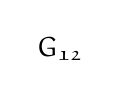
\begin{tikzpicture}[baseline=(current bounding box.center)]
    \begin{feynman}
        \vertex {$G_{\mathfrak{12}}$};
    \end{feynman}
\end{tikzpicture}
\begin{tikzpicture}[baseline=(current bounding box.center)]
    \begin{feynman}
        \vertex {$=$};
    \end{feynman}
\end{tikzpicture}
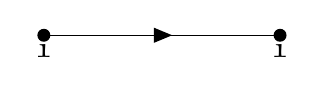
\begin{tikzpicture}[baseline=(current bounding box.center)]
	\begin{feynman}
		\vertex[dot] (a) {};
		\vertex[dot, right=3cm of a] (b) {};
		
		\node [below=0.2cm of a] {$\mathfrak{1}$};
		\node [below=0.2cm of b] {$\mathfrak{1}$};
		
		\diagram* {
			(a) -- [fermion] (b)
		};	
	\end{feynman}
\end{tikzpicture}

\end{document}